\pdfoutput=1
\documentclass[11pt,a4paper]{article}
\usepackage[preprint]{papertwocol}
\usepackage{times,latexsym}
\usepackage[T1]{fontenc}
\usepackage[utf8]{inputenc}
\usepackage{microtype}
\usepackage{amsmath,amssymb,booktabs,tabularx,array}
\usepackage{graphicx}
\usepackage{colortbl}
\definecolor{tablegray}{gray}{0.92}
\usepackage{enumitem}
\usepackage{url}
\newcolumntype{L}{>{\raggedright\arraybackslash}X}
\newcommand{\bench}{S1CogBench}
\newcommand{\pending}{\textit{Pending}}
\title{S1CogBench: What System One Decision Models Can and Cannot Do on Cognitive Experiments}
\author{Dengzhe Hou\textsuperscript{1,*}\qquad Kazunori D Yamada\textsuperscript{1}\\[3pt]
{\normalfont \textsuperscript{1}Tohoku University}\\[3pt]
{\normalfont\small \textsuperscript{*}Corresponding author.\quad Project: \href{https://github.com/dengzhe-hou/S1CogBench}{\texttt{github.com/dengzhe-hou/S1CogBench}}}}
\date{}
\begin{document}
\raggedbottom
\maketitle
\begin{abstract}
Language models are no longer used only to generate text. Software also asks them for decisions, in routing, guardrails, and automated gates. System One decision models, also called typed decision models, such as Jev and Laya, return one fast decision over the legal options, leaving no text to inspect. However, a fast, well-formed decision does not show that the model used the evidence. Cognitive experiments can test this, because they vary task demands and measure how behavior changes, yet existing cognitive benchmarks evaluate language and multimodal models. We introduce \bench{} to ask what these models can and cannot do on 24 cognitive tasks, evaluating five open models and Jev and keeping conditions and scoring apart from disclosed adaptations. We find that decision models vary widely in reliability, acting well does not imply predicting humans, aggregate scores hide how decisions respond to conditions, and speed comes mainly from answering without generation. To our knowledge, \bench{} is the first benchmark of System One decision models on established cognitive experiments, and it gives a shared test of whether their decisions respond to evidence, feedback, memory load, and future opportunities before software relies on them.

\end{abstract}
\section{Introduction}
\label{sec:introduction}
Jev, Laya, and Intern-Decision exemplify a shift from free text generation to structured decisions \citep{typesafeJev,convaiLaya,internlm2026decision}. They return one typed decision over the legal options in a single call, so software can act on it directly for routing, guardrails, and automated gates \citep{zhuang2026decisionpivot,rafe2026systemone}, and a small model of this kind can be invoked many times inside a larger system. We call them \emph{System One decision models} \citep{typesafeJev}, also called typed decision models \citep{sun2026typesafe,sharma2026typedbench}, as an operational label. We take their speed as a premise and measure where it comes from.

\begin{figure*}[!t]
\centering
\setlength{\abovecaptionskip}{4pt}
\makebox[\textwidth][c]{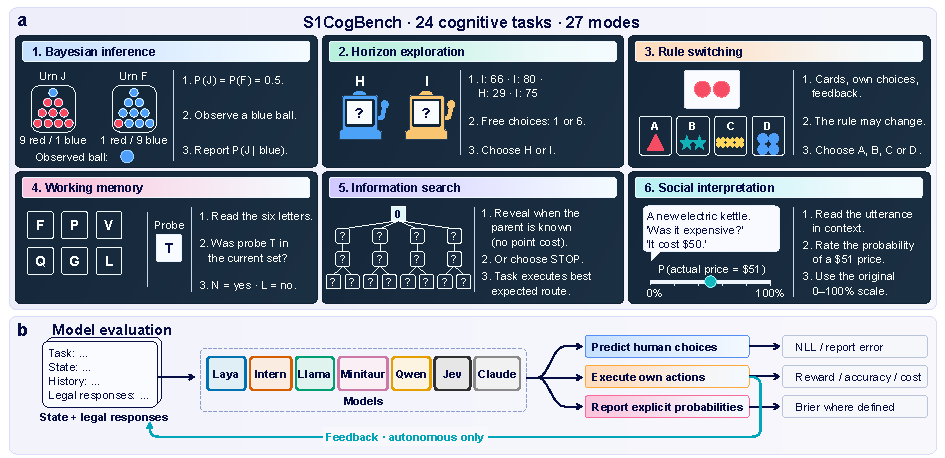
\includegraphics[width=\textwidth,pagebox=cropbox]{figures/fig1.pdf}}
\caption{\textbf{S1CogBench connects cognitive tasks to model evaluation.}
\textbf{(a)} Six representative tasks from the 24-task, 27-mode suite.
\textbf{(b)} Adapters supply visible states, histories, and legal responses to the models, and each output has its own score. Model-specific coverage and API configurations are recorded in Appendix~\ref{app:selected-api-extension}.}
\label{fig:framework}
\vspace{-12pt}
\end{figure*}


A typed interface makes a response easy to execute, but it does not show that the response uses the relevant evidence, and no generated text is left to inspect \citep{sharma2026typedbench}. A model can return a well-formed distribution yet ignore feedback or stop searching too early. In closed-loop environments small System One models rarely succeed \citep{chen2026system1arena}, but such environments do not isolate which demand fails. Cognitive experiments can, because they manipulate information, uncertainty, memory load, incentives, or future opportunities and show how behavior changes.

Existing cognitive benchmarks evaluate language and multimodal models \citep{codaforno2024cogbench,binz2025centaur,ying2026coggym,nie2025evolve,hou2026cogarena}, and CogGym's 50 models include no System One decision model. System1-Arena does evaluate System One decision models, but on static decision tasks and agent environments \citep{chen2026system1arena}. To our knowledge, \bench{} is the first benchmark to evaluate System One decision models on established cognitive experiments.

We ask what these models can and cannot do on these experiments. RQ1 asks whether a model that acts well also predicts humans. RQ2 asks what overall scores hide about how behavior changes across conditions. RQ3 asks where the speed comes from.

Four findings answer these questions.
\begin{itemize}[leftmargin=*,itemsep=1pt,topsep=2pt]
\item Decision models vary widely in reliability. Laya does not beat uniform choice on 17 of 26 targets, against 3 for Intern-Decision, which also beats the Qwen3.5 backbone it is fine-tuned from on 23, the one pair we can compare (Section~\ref{sec:main-results}).
\item Acting well does not imply predicting humans (RQ1). In Mouselab, Qwen has the highest autonomous reward but predicts humans worse than uniform choice, and Laya has the best NLL of the open models with zero reward (Section~\ref{sec:rq1}).
\item Aggregate scores hide condition effects (RQ2), as Horizon, the Wisconsin Card Sorting Test (WCST), and reinforcement learning and working memory (RLWM) show (Section~\ref{sec:rq2}).
\item Speed comes mainly from the interface (RQ3). Under the same readout, Intern-Decision is no faster than its same-size backbone, while generation takes 80 to 316 times as long as one forward pass in the two general models we timed (Section~\ref{sec:rq3}).
\end{itemize}

\bench{} is built for models that return a fast decision in a single call. It turns each of 24 tasks into a typed request over legal options, scores option probabilities and native choices, times each decision with generation as a control, and supports new model adapters.

\section{Related work}
\label{sec:related}
Cognitive benchmarks evaluate language and multimodal models. CogBench uses ten behavioral metrics from seven experiments \citep{codaforno2024cogbench}, CogGym evaluates 50 models on 258 single-turn experiments \citep{ying2026coggym}, and Psych-101 and Centaur evaluate held-out human-response prediction and feed model-generated choices back into Horizon and Two-step \citep{binz2025centaur}. CogArena studies the consistency and predictive validity of cognitive measurements \citep{hou2026cogarena}, and WMF-AM probes cumulative state tracking \citep{hou2026wmfam}. \citet{namazova2025centaur} compare predictive and generative behavior, and \bench{} extends this distinction to explicit event probabilities, source-defined condition effects, and structured interfaces.

System1-Arena compares System One decision models through typed probability requests, closed-loop environments, latency, and cost \citep{chen2026system1arena}, and TypedBench examines calibration, wording and option sensitivity, length, and asymmetric decision costs \citep{sharma2026typedbench}. These works already provide unified interfaces, conditional diagnostics, and efficiency measurement. Table~\ref{tab:direct-benchmark-comparison} compares the closest resources with ours, and Appendix~\ref{app:related} covers further work.

\begin{table*}[!t]
\centering\small
\begin{tabular}{@{}lccccc@{}}
\toprule
Resource & \begin{tabular}[b]{@{}c@{}}Cognitive\\experiments\end{tabular} & \begin{tabular}[b]{@{}c@{}}Predicts human\\responses\end{tabular} & \begin{tabular}[b]{@{}c@{}}Closed-loop\\actions\end{tabular} & \begin{tabular}[b]{@{}c@{}}System One\\models\end{tabular} & \begin{tabular}[b]{@{}c@{}}Decision time\\or cost\end{tabular} \\
\midrule
CogBench \citep{codaforno2024cogbench} & 7 & -- & $\checkmark$ & -- & -- \\
CogGym, Sept.~2026 v1 \citep{ying2026coggym} & 258 & $\checkmark$ & -- & -- & -- \\
Psych-101 / Centaur \citep{binz2025centaur} & 160 & $\checkmark$ & ($\checkmark$) & -- & -- \\
CogArena \citep{hou2026cogarena} & 13 & -- & -- & -- & -- \\
BanditBench / EVOLvE \citep{nie2025evolve} & -- & -- & $\checkmark$ & -- & -- \\
System1-Arena \citep{chen2026system1arena} & -- & -- & $\checkmark$ & $\checkmark$ & $\checkmark$ \\
TypedBench \citep{sharma2026typedbench} & -- & -- & -- & $\checkmark$ & $\checkmark$ \\
DecisionPivot \citep{zhuang2026decisionpivot} & -- & -- & -- & $\checkmark$ & -- \\
\midrule
\rowcolor{tablegray} \textbf{\bench{}} & \textbf{24} & $\checkmark$ & $\checkmark$ & $\checkmark$ & $\checkmark$ \\
\bottomrule
\end{tabular}
\caption{Coverage of the closest evaluation resources in each paper's main evaluation. Counting units differ across resources, and ($\checkmark$) marks selected tasks only. This compares coverage, not scores.}
\label{tab:direct-benchmark-comparison}
\end{table*}


\section{The \bench{} benchmark}
\label{sec:benchmark}
\bench{} maps an original cognitive experiment to the information visible at each decision, its legal responses, a model output, a readout, and source-grounded scores. Figure~\ref{fig:framework} summarizes this connection.

\subsection{Task selection and provenance}
The 24 tasks fall into ten organizational domains (Table~\ref{tab:domains}). WCST, Horizon, and Mouselab each have a human-prediction and an autonomous mode, giving 27 modes. Appendix~\ref{app:tasks} lists all 24 tasks and their sources. Each specification identifies the original study, adopted public dataset or environment version, manipulation, stimuli, legal responses, feedback, reset and stopping rules, and scoring unit. The 24 tasks come from published experiments and benchmarks, such as Horizon \citep{wilson2014exploration}, WCST \citep{grant1948cardsorting}, RLWM \citep{collins2012rlwm}, Mouselab \citep{callaway2022planning}, and the two-step task \citep{daw2011model}. Official splits are used where provided. Inclusion follows complementary manipulations and interface compatibility, independently of observed model rankings.

\begin{table*}[t]
\centering\footnotesize
\begin{tabularx}{\linewidth}{@{}lLL@{}}
\toprule
Domain & Tasks & What the experiments vary \\
\midrule
Evidence & Bayesian urn, multiple-cue judgment, multi-attribute choice, probability coherence & Prior probability, likelihood, cue validity, coherence \\
Categories & SHJ, Medin, weather prediction & Category structure, feedback, transfer and typicality \\
History & RLWM, recent probes & Set size, repetition interval, recent interference \\
Adaptation & WCST, restless bandit, instrumental learning & Rule changes, changing rewards, outcome feedback \\
Exploration & Horizon, stationary bandits & Future opportunities, uncertainty \\
Information & Hybrid sampling, Mouselab & Reveal actions, sampling cost, stopping conditions \\
Preference & BART, temporal discounting & Risk, reward magnitude, explicit delays \\
Planning & Two-step & Transitions, changes in outcome value \\
Social & False-belief QA, politeness, pragmatic interpretation, nonliteral number & Belief access, communicative goals, literal meaning \\
Metacognition & Self-assessment & Difficulty, correctness \\
\bottomrule
\end{tabularx}
\caption{The 24 tasks in ten organizational domains. Domains organize the tasks and are not validated latent factors. Appendix~\ref{app:tasks} gives each task\textquotesingle{}s source.}
\label{tab:domains}
\end{table*}

\subsection{Typed decision interface}
For each decision, an adapter gives the model what the original task shows at that point, the history $h_t$ as a visible state $x_t$, and the ordered legal responses $\mathcal A_t$. For human prediction the history is the participant's, and for autonomous execution it is the model's own. Histories can be complete, summarized, windowed, or absent, and these are different information conditions. Responses can be categorical actions, ordinal ratings, numerical reports, or event probabilities.

The model returns a distribution $p_\theta(a\mid x_t,\mathcal A_t)$ over those responses. A readout is the rule that turns this output into a probability or an executed action, such as a native choice, a sampled action, or generative decoding. We record the distribution, the native choice, the executed action, the feedback, and the timing, so a model's distribution stays separate from randomness added at execution. An episode ends as in the original task, for example after a fixed number of trials, an explicit stop, or a terminal state.

Text displays, supplied histories, and constrained response sets are disclosed adaptations of the original tasks. Hybrid sampling supplies the authors' posterior summary, autonomous Mouselab has zero observation cost and picks the final route by expected value, and stationary bandits use the summary-history context of the original code, which exposes counts and mean rewards rather than the raw history.

\subsection{Scoring targets}
For observed participant $i$ and scored trial $t$, human-response NLL scores the observed choice given its preceding history, using each source's response set and its participant, fold, or response weighting,
\begin{equation}
 \operatorname{NLL}=-\frac{1}{N}\sum_{i,t}\log p_\theta(a_{it}\mid h_{it}).
 \label{eq:nll}
\end{equation}
NLL over the legal responses and NLL over the full vocabulary are different scores. A returned zero gives infinite NLL unless the primary metric of the source scorer defines an epsilon, as in WCST and Horizon.

Autonomous scores use executed trajectories, with total reward
\begin{equation}
 G=\sum_t(r_t-c_t),
 \label{eq:return}
\end{equation}
where the reward, each cost, and the horizon follow the source environment. Single-event Brier $(q-Y)^2$ needs an explicit probability and an observed event. Answer-category Brier sums over categories, so the two are not on the same scale.

We report nine shared measures, accuracy, reward, pseudo-regret, MAE, human NLL, Brier, latency P50 and P95, and invalid-response rate, each where the task defines it. Per-mode definitions and tables, complete curves, per-target API records, and reference details are in the project repository. Original cognitive effects are reported alongside these scores. Uncertainty uses participants or independent environments, not trajectory steps, and paired 95\% intervals state their resampling unit.

\subsection{References}
Source-defined uniform controls are available for 26 performance targets, with varying legal supports and the original tie credit. References are fits to participants on 16 targets, other participants\textquotesingle{} responses on 5, policies without human fitting on 4, and analytic solutions or answer keys on 2, and Appendix~\ref{app:protocol} gives each one\textquotesingle{}s fitting exposure and implementation.

\section{Experiments}
\label{sec:results}
\begin{table*}[!t]
\centering\footnotesize
\setlength{\tabcolsep}{0pt}
\begin{tabular*}{\linewidth}{@{\extracolsep{\fill}}l r rrrrr@{\hspace{12pt}}rr@{\hspace{12pt}}r@{}}
\toprule
 & & \multicolumn{5}{c}{Open models} & \multicolumn{2}{c}{API models} & \\
\cmidrule(lr){3-7}\cmidrule(lr){8-9}
Task & Uniform & Laya & Intern & Llama & Minitaur & Qwen & Jev & Haiku & Reference \\
\midrule
\multicolumn{10}{@{}>{\columncolor{tablegray}}l}{\textit{Human-response NLL $\downarrow$}} \\
Multiple-cue judgment & 2.197 & \textcolor{gray}{2.342} & \textbf{1.570} & \textcolor{gray}{2.687} & 1.984 & \textcolor{gray}{3.012} & $+\infty$ & -- & 2.029 \\
Multi-attribute choice & 0.693 & \textcolor{gray}{0.730} & \textbf{0.546} & \textcolor{gray}{0.786} & \textcolor{gray}{0.722} & 0.613 & 0.329 & 0.206 & 0.192 \\
WCST & 1.386 & \textcolor{gray}{1.462} & 1.378 & \textcolor{gray}{1.431} & \textbf{1.344} & \textcolor{gray}{1.968} & 1.543 & -- & 0.840 \\
Horizon & 0.693 & \textcolor{gray}{0.702} & 0.518 & 0.503 & \textbf{0.409} & 0.661 & 0.414 & 0.390 & 0.400 \\
Hybrid sampling & 1.386 & \textcolor{gray}{1.390} & 1.116 & \textcolor{gray}{1.515} & \textbf{1.039} & \textcolor{gray}{2.648} & $+\infty$ & -- & 0.264 \\
Mouselab & 1.634 & \textbf{\textcolor{gray}{1.717}} & \textcolor{gray}{2.109} & \textcolor{gray}{2.743} & \textcolor{gray}{2.125} & \textcolor{gray}{2.464} & 1.458 & -- & 1.367 \\
Politeness & 1.014 & \textcolor{gray}{1.192} & \textbf{0.799} & \textcolor{gray}{1.584} & 1.008 & 1.000 & $+\infty$ & $+\infty$ & 0.587 \\
Pragmatic interpretation & 1.282 & \textcolor{gray}{1.592} & \textbf{0.814} & \textcolor{gray}{1.851} & 1.049 & 1.240 & $+\infty$ & $+\infty$ & 0.416 \\
Self-assessment & 2.039 & \textcolor{gray}{$+\infty$} & 2.029 & \textcolor{gray}{2.523} & \textbf{1.885} & \textcolor{gray}{2.262} & $+\infty$ & -- & 1.619 \\
\midrule
\multicolumn{10}{@{}>{\columncolor{tablegray}}l}{\textit{Accuracy under given histories (\%) $\uparrow$}} \\
SHJ categories & 50.0 & \textcolor{gray}{50.0} & 65.0 & 52.9 & 54.5 & \textbf{71.3} & 87.4 & 91.2 & 93.8 \\
Medin categories & 50.0 & \textcolor{gray}{49.6} & \textbf{72.3} & 53.5 & 55.9 & 53.8 & 86.8 & 97.4 & 96.6 \\
Weather prediction & 50.0 & 54.5 & \textbf{73.0} & \textcolor{gray}{47.5} & 53.8 & 50.5 & 80.8 & 80.2 & 78.2 \\
RLWM & 33.3 & 34.9 & \textbf{77.8} & 41.7 & 49.0 & 59.3 & 89.5 & 89.4 & 89.3 \\
Recent probes & 50.0 & \textcolor{gray}{49.7} & \textbf{82.1} & 55.6 & \textcolor{gray}{49.5} & 53.5 & 99.0 & 100.0 & 100.0 \\
False-belief QA & 50.0 & \textcolor{gray}{39.5} & 82.5 & 81.8 & 65.0 & \textbf{82.8} & 71.5 & 82.6 & 100.0 \\
\midrule
\multicolumn{10}{@{}>{\columncolor{tablegray}}l}{\textit{Autonomous choices, correct or optimal (\%) $\uparrow$}} \\
WCST & 25.0 & 25.5 & 27.9 & \textbf{31.4} & 28.2 & 25.2 & 28.5 & -- & 48.9 \\
Restless bandit & 50.0 & 55.4 & \textbf{65.6} & 57.1 & \textcolor{gray}{49.0} & 50.5 & 63.9 & -- & 68.8 \\
Instrumental learning & 75.0 & \textcolor{gray}{73.9} & 81.4 & 79.2 & \textbf{86.7} & 80.0 & 86.7 & -- & 94.9 \\
Horizon & 50.0 & 54.8 & \textbf{78.7} & 66.4 & 71.7 & 63.3 & 82.9 & -- & 74.6 \\
Stationary bandits & 12.5 & 17.6 & \textbf{37.4} & 13.5 & \textcolor{gray}{9.8} & 28.9 & 47.0 & -- & 68.1 \\
\midrule
\multicolumn{10}{@{}>{\columncolor{tablegray}}l}{\textit{Autonomous reward $\uparrow$}} \\
Mouselab & 7.01 & \textcolor{gray}{0.00} & \textcolor{gray}{0.00} & \textcolor{gray}{3.77} & \textcolor{gray}{0.00} & \textbf{17.40} & 8.21 & -- & 11.77 \\
BART & 0.84 & \textcolor{gray}{0.00} & \textbf{\textcolor{gray}{0.74}} & \textcolor{gray}{0.28} & \textcolor{gray}{0.00} & \textcolor{gray}{0.00} & 1.76 & 6.27 & 10.49 \\
Two-step & 0.50 & 0.50 & \textbf{0.52} & 0.50 & 0.51 & 0.52 & 0.55 & 0.55 & 0.52 \\
\midrule
\multicolumn{10}{@{}>{\columncolor{tablegray}}l}{\textit{Report error (MAE) $\downarrow$}} \\
Bayesian urn & 0.349 & 0.291 & \textbf{0.235} & 0.240 & 0.294 & 0.246 & 0.068 & 0.001 & 0.000 \\
Probability coherence & 32.13 & \textcolor{gray}{32.98} & \textbf{18.95} & 28.57 & 19.04 & 21.87 & 17.66 & -- & 16.54 \\
Nonliteral number & 34.77 & 30.86 & \textbf{16.87} & 25.10 & 28.53 & 29.75 & 20.37 & 22.52 & 4.98 \\
\midrule
\multicolumn{10}{@{}>{\columncolor{tablegray}}l}{\textit{Preference, later reward chosen (\%)}} \\
Temporal discounting & 50.0 & 0.0 & 16.7 & 0.0 & 80.0 & 90.0 & 50.0 & 77.8 & 41.5 \\
\bottomrule
\end{tabular*}
\caption{Primary targets of the 27 modes, grouped by what is scored. Arrows show the better direction. Bold marks the best of the five open models, gray marks scores not better than Uniform, a dash means no complete score, and $+\infty$ means zero probability on a human choice under a scorer with no epsilon. Reference is a task-specific baseline, such as a fit to human data or an analytic solution. Open models keep their original readouts (Appendix~\ref{app:protocol}), and Haiku\textquotesingle{}s NLL uses stated probabilities. Appendix~\ref{app:table2-controls} gives reference types and the reason for each dash, and Appendix~\ref{app:selected-api-extension} gives Opus and Sonnet.}
\label{tab:task-summary}
\end{table*}

\subsection{Setup}
\label{sec:protocol}
We evaluate five open models as released. Laya English, a non-autoregressive model built on ModernBERT, and Intern-Decision-4B are System One decision models. Intern-Decision is fine-tuned from Qwen3.5-4B~\citep{qwen35_4b} for structured decisions, which we call decision training, so Qwen is its backbone comparison. Llama-3.1-8B-Instruct~\citep{grattafiori2024llama3} is a general-purpose control, and Minitaur-8B~\citep{binzMinitaur} is trained on human behavior. Their training data and compute are not matched. All 120 task--model pairs run on the full sample, and only multiple-cue judgment uses a compact history.

Jev, available only through its API, runs all 27 modes, and Claude5.5, a general model with adaptive thinking, runs selected tasks because of cost (Appendix~\ref{app:selected-api-extension}).

To separate models from readouts, we also run all five models on Horizon and WCST under both legal argmax and sampling.

\subsection{Main results}
\label{sec:main-results}
Table~\ref{tab:task-summary} gives one primary target for each of the 27 task modes. Laya is not better than uniform choice on 17 of 26 targets, followed by Llama on 11, Minitaur on 7, Qwen on 6, and Intern-Decision on 3. Intern-Decision has the best score of the five models on 16 targets and beats its Qwen3.5 backbone on 23. The remaining mode, temporal discounting, reports how often the later reward is chosen, a preference with no better direction.

\subsection{Does acting well imply predicting humans? (RQ1)}
\label{sec:rq1}
\begin{figure*}[t]
\centering
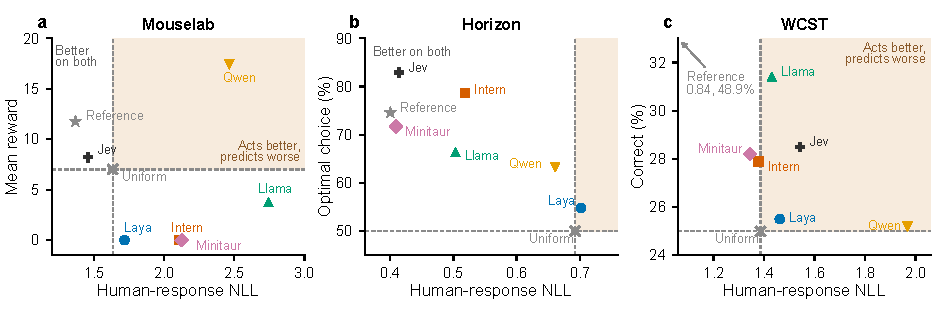
\includegraphics[width=\textwidth]{figures/fig2.pdf}
\caption{Human prediction against autonomous score under the original readouts, from Table~\ref{tab:task-summary}. Dashed lines mark uniform choice, so the upper-left region beats it on both scores and the shaded region acts better but predicts worse. Panel c is zoomed, with Reference off scale. Points are not paired on the same decisions across the two axes.}
\label{fig:rq1-targets}
\end{figure*}

Figure~\ref{fig:rq1-targets} plots acting against predicting humans for the three tasks that have both modes. Mouselab separates the two most clearly. In this search task a model reveals tree nodes or stops, and the task then takes the path with the best expected value. We set the observation cost to zero, whereas the human data come from the original waiting-time protocol, so the two modes also differ in cost. Intern, Laya, and Minitaur stop immediately in all 23,750 episodes, so their reward is zero. Qwen reveals 15.5 nodes per episode and reaches 17.40, above the 11.77 of MetaGreedy, a one-step value-of-information policy replayed on the same trees (Appendix~\ref{app:new-traditional-references}). These are terminal expected values, not realized path rewards. Human prediction gives a different answer. Qwen's NLL is 2.464, all five models are worse than the 1.634 of uniform choice, and Laya is best at 1.717 with zero reward.

Horizon and WCST separate the two less clearly, and only under the original readouts. Among the five open models in Horizon (Table~\ref{tab:p3-final-horizon}), the two scores mostly agree, although Minitaur has the lowest NLL (0.409) and Intern-Decision the highest reward (54.93). Under one shared readout, Minitaur also has the highest reward. A three-parameter Rescorla-Wagner (RW) fit to 25 training participants scores NLL 0.400 and reward 54.56. In WCST, Minitaur predicts best (NLL 1.344), whereas Llama acts best (31.4\%) but predicts worse than uniform (1.431 against 1.386). A shared argmax puts Minitaur first at 34.3\%.

Probability scores also select different models. Among the open models in Bayesian urn inference, Intern has the lowest posterior MAE over 400 generated queries (0.2345), whereas Qwen has the lowest event Brier error (0.2299).

\begin{table}[!b]
\centering\footnotesize
\setlength{\tabcolsep}{1.6pt}
\begin{tabular}{@{}lrrrrrrr@{}}
\toprule
 & Human & \multicolumn{3}{c}{Mean reward} & \multicolumn{3}{c}{Optimal choice (\%)} \\
\cmidrule(lr){3-5}\cmidrule(lr){6-8}
Model & NLL & orig. & argmax & sample & orig. & argmax & sample \\
\midrule
\rowcolor{tablegray} Uniform & 0.693 & 50.0 & 50.0 & 50.0 & 50.0 & 50.0 & 50.0 \\
Laya & 0.702 & 51.0 & 51.8 & 51.0 & 54.8 & 57.9 & 54.8 \\
Intern & 0.518 & \textbf{54.9} & 54.9 & 52.2 & \textbf{78.7} & 78.7 & 62.8 \\
Llama & 0.503 & 52.9 & 53.6 & 52.7 & 66.4 & 70.9 & 65.2 \\
Minitaur & \textbf{0.409} & 53.9 & \textbf{56.2} & \textbf{53.7} & 71.7 & \textbf{84.0} & \textbf{70.9} \\
Qwen & 0.661 & 52.2 & 52.2 & 51.8 & 63.3 & 63.3 & 60.8 \\
\rowcolor{tablegray} RW fit & 0.400 & 54.6 & 56.0 & 54.6 & 74.6 & 84.9 & 74.6 \\
\bottomrule
\end{tabular}
\caption{Horizon prediction of six held-out participants (NLL over legal responses, 6,720 free choices) and autonomous play on 31 source timelines (34,720 free choices per model and readout). Orig. is each model's own readout, argmax for Intern and Qwen and sampling for the others. Within a model, only the readout changes across columns. Bold marks the best open model in each column.}
\label{tab:p3-final-horizon}
\end{table}


Jev scores at or near the top in RLWM and autonomous Horizon. It reaches 89.5\% in RLWM under human-block histories, level with the 89.3\% of the same-participant fitted reference under argmax, and 82.9\% optimal choices in Horizon, between that task's human-fitted reference at 74.6\% under sampling and 84.9\% under greedy replay. Its two-decimal probabilities, however, give zero mass to some human choices, so its NLL is infinite on five of its nine prediction targets (Appendix~\ref{app:selected-api-extension}). None of those five has an autonomous mode. Where both modes exist, Jev beats uniform on both in Horizon and Mouselab (NLL 0.414 and 1.458). In WCST its NLL (1.543) is worse than uniform and its accuracy (28.5\%) is close to it.

\subsection{What do aggregate scores hide? (RQ2)}
\label{sec:rq2}
Horizon shows a response to future opportunities that the pooled NLL misses. When more choices remain (horizon 6 against 1), humans choose the less-observed arm 10.00 percentage points more often at their first unequal-information free choice. Under the same histories, models predict changes of only $-0.49$ to $1.18$ points (Figure~\ref{fig:exploratory-cognitive-profiles}a).

\begin{figure*}[t]
\centering
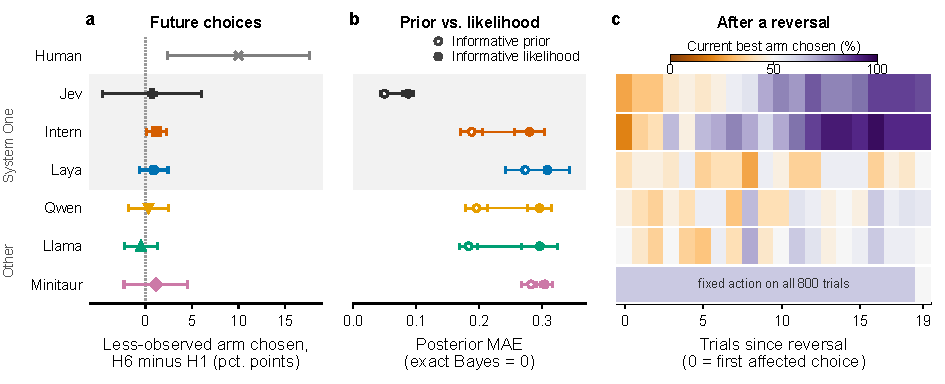
\includegraphics[width=\textwidth]{figures/fig3.pdf}
\caption{Cognitive profiles. (a) Predicted change in choosing the less-observed arm between horizons 6 and 1 under human histories. (b) Posterior MAE with a more informative prior or likelihood. (c) Choices aligned to reversals, as means over 10 runs. Minitaur selected arm F on all 800 trials, so its flat row is not adaptation. Error bars are 95\% Student-t intervals over six participants (a) and 200 paired seeds (b), uncorrected for multiple comparisons. Panels b and c have no human data.}
\label{fig:exploratory-cognitive-profiles}
\end{figure*}

In WCST, fewer perseveration errors can accompany worse accuracy. Laya makes them on 15.24\% of trials against 28.82\% for Llama, but its autonomous accuracy is also lower (25.47\% against 31.39\%), and its rate is close to the 17.13\% of uniform choice, so this rate alone cannot rank flexibility (Table~\ref{tab:wcst}). All five autonomous accuracies lie between 25.20\% and 31.39\%, close to the 25\% of uniform choice and far below the 50.00\% of humans, and the sequential-learning (SL) reference reaches 48.92\%. On 74 common decisions from two source participants, Claude models with adaptive thinking reach 63.51 to 66.22\%, against 18.92 to 43.24\% for the open models under shared legal readouts (Table~\ref{tab:claude-common-source}). So the text conversion supports learning from feedback and does not alone explain the near-chance open-model scores.

In RLWM, average accuracy does not predict the load effect (Table~\ref{tab:rlwm-models}). Qwen averages 59.39\% and loses 20.34 points from set size 2 to 6, whereas Minitaur averages 49.09\% and loses 11.34, and Intern averages 77.83\% and loses 11.37, both close to the 12.74 of humans. Learning follows average accuracy more closely (Figure~\ref{fig:rlwm-curves}). From presentation 1 to 10 at set size 6, Intern gains 61.49 points, more than the 46.35 of humans, because it starts below them and ends above them. Laya stays flat, gaining only 0.21.

\begin{table}[!h]
\centering\footnotesize
\setlength{\tabcolsep}{3pt}
\begin{tabular}{@{}lrrrrr@{}}
\toprule
 & \multicolumn{2}{c}{Human history} & \multicolumn{3}{c}{Autonomous} \\
\cmidrule(lr){2-3}\cmidrule(lr){4-6}
Model & Accuracy & NLL & Accuracy & Persev. & Set-loss \\
\midrule
\rowcolor{tablegray} Human & 50.00 & -- & 50.00 & 7.32 & 1.88 \\
\rowcolor{tablegray} Uniform & 25.00 & 1.3863 & 25.00 & 17.13 & 17.13 \\
Laya & 25.53 & 1.4616 & 25.47 & 15.24 & 18.16 \\
Intern & 28.90 & 1.3781 & 27.90 & 21.25 & 15.84 \\
Llama & \textbf{32.56} & 1.4307 & \textbf{31.39} & 28.82 & 13.78 \\
Minitaur & 30.06 & \textbf{1.3435} & 28.16 & 21.85 & 14.61 \\
Qwen & 25.07 & 1.9677 & 25.20 & 15.88 & 17.88 \\
\rowcolor{tablegray} SL refit & 60.40 & 0.8402 & 48.92 & 9.47 & 4.63 \\
\bottomrule
\end{tabular}
\caption{WCST means over 75 held-out participants (12,754 trials per mode). Accuracy and error rates are percentages of all trials. Persev. is a wrong choice that repeats the rule of a wrong previous choice, and Set-loss is a wrong choice that leaves the rule of a correct one. SL is a sequential-learning model fitted to the other 300 participants. NLL uses the source $-\log(p+10^{-12})$, and invalid outputs stay in the denominators. Bold marks the best of the five models in the first three columns.}
\label{tab:wcst}
\end{table}


In Bayesian urn inference, overall MAE hides a difference between conditions. All five models have higher error when the likelihood is the more informative input than when the prior is (0.28 to 0.31 against 0.18 to 0.28, Figure~\ref{fig:exploratory-cognitive-profiles}b).

\begin{table}[!b]
\centering\footnotesize
\setlength{\tabcolsep}{4pt}
\begin{tabular}{@{}lrrrr@{}}
\toprule
 & \multicolumn{2}{c}{Horizon reward} & \multicolumn{2}{c}{WCST correct (\%)} \\
\cmidrule(lr){2-3}\cmidrule(lr){4-5}
Model & argmax & sample & argmax & sample \\
\midrule
\rowcolor{tablegray} Opus & \multicolumn{2}{c}{56.87} & \multicolumn{2}{c}{63.51} \\
\rowcolor{tablegray} Sonnet & \multicolumn{2}{c}{56.95} & \multicolumn{2}{c}{66.22} \\
\rowcolor{tablegray} Haiku & \multicolumn{2}{c}{56.86} & \multicolumn{2}{c}{66.22} \\
Laya & 50.23 & 50.05 & 20.27 & 22.97 \\
Intern & 56.22 & 51.35 & 33.78 & 29.73 \\
Llama & 54.33 & 51.57 & 37.84 & 39.19 \\
Minitaur & 56.48 & 52.92 & 43.24 & 27.03 \\
Qwen & 52.68 & 51.33 & 18.92 & 22.97 \\
\bottomrule
\end{tabular}
\caption{Saved decisions on common source identities, 200 Horizon free choices from one timeline and 74 WCST decisions from two participants. Claude answers in a final line of text with adaptive thinking, so the readouts are not matched, and Haiku\textquotesingle{}s two invalid WCST attempts count as wrong. Each row keeps its own action-dependent history.}
\label{tab:claude-common-source}
\end{table}


In the Restless bandit, a flat curve can reflect a fixed action rather than adaptation. Minitaur chooses arm F on all 800 trials, although its probability of F varies from 0.5622 to 0.9325, so its curve in Figure~\ref{fig:exploratory-cognitive-profiles}c reflects a constant action and the environment. Jev and Intern-Decision instead change after a reversal. They choose the current best arm on 36.7\% and 42.0\% of the first five trials after a reversal and on 85.0\% and 91.3\% of trials 15 to 19, whereas Laya, Llama, and Qwen reach 46.0\%, 54.7\%, and 55.0\%.

\begin{figure}[!b]
\centering
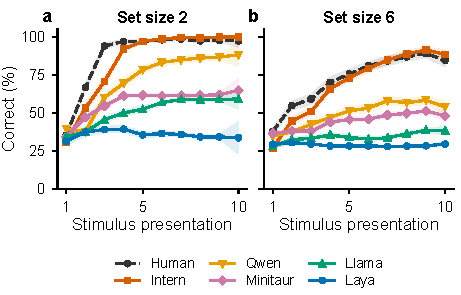
\includegraphics[width=\columnwidth]{figures/fig4.pdf}
\caption{RLWM correct responses by stimulus presentation under complete human-block histories, with pointwise 95\% Student-t intervals across participants (34 at set size 2 and 69 at set size 6 by presentation 10).}
\label{fig:rlwm-curves}
\end{figure}


\begin{table}[t]
\centering\scriptsize
\setlength{\tabcolsep}{3pt}
\begin{tabular}{@{}lrrr@{}}
\toprule
 & Overall & Size 6 minus 2 & Pres. 10 minus 1 \\
Source & (\%, $n=79$) & (pp, $n=79$) & size 6 (pp, $n=69$) \\
\midrule
\rowcolor{tablegray} Human & 80.24 & $-$12.74 [$-$14.54, $-$10.99] & +46.35 [41.13, 51.53] \\
\rowcolor{tablegray} Uniform & 33.33 & +0.00 & +0.00 \\
Laya & 34.85 & $-$7.17 [$-$8.53, $-$5.79] & +0.21 [$-$2.46, 2.69] \\
Intern & 77.83 & $-$11.37 [$-$12.80, $-$9.96] & +61.49 [58.09, 64.84] \\
Llama & 41.78 & $-$16.73 [$-$17.94, $-$15.46] & +10.49 [7.27, 13.62] \\
Minitaur & 49.09 & $-$11.34 [$-$12.58, $-$10.12] & +11.10 [7.34, 15.11] \\
Qwen & 59.39 & $-$20.34 [$-$22.21, $-$18.41] & +19.75 [15.71, 23.87] \\
\bottomrule
\end{tabular}
\caption{RLWM prediction of all 52,911 eligible responses from 79 participants under complete human-block histories. Accuracy uses the hidden correct action, and means weight participants equally, whereas Table~\ref{tab:task-summary} weights responses. Pres. means presentation, and contrasts pair the participants shown in the header. Brackets are pointwise 95\% participant-bootstrap intervals (5,000 resamples, uncorrected).}
\label{tab:rlwm-models}
\end{table}


\begin{table}[!b]
\centering\footnotesize
\setlength{\tabcolsep}{2pt}
\begin{tabular}{@{}lrrrr@{}}
\toprule
 & & E2E P50 & Ratio to & Largest \\
Config. & Requests & (ms) & Llama & P95 (ms) \\
\midrule
Laya FP32 & 5,576 & 25.50--274.44 & 0.67--0.95 & 742.54 \\
Laya BF16 & 5,576 & 26.55--82.18 & 0.23--0.71 & 200.76 \\
Laya fast & 1,200 & 6.45--59.83 & 0.12--0.17 & 50,395 \\
Intern FLA & 5,576 & 52.06--219.40 & 0.75--1.41 & 437.76 \\
Intern Torch & 1,200 & 174.58--655.74 & 2.19--4.70 & 1,223 \\
Qwen FLA & 5,576 & 51.66--211.88 & 0.71--1.40 & 427.38 \\
Qwen Torch & 1,200 & 162.25--595.82 & 2.09--4.40 & 1,189 \\
\rowcolor{tablegray} Llama & 5,576 & 36.97--274.02 & 1.00 & 611.22 \\
Minitaur & 5,576 & 35.65--265.50 & 0.93--0.97 & 596.42 \\
\bottomrule
\end{tabular}
\caption{Controlled latency over six task modes, on one A100 at batch size one. Ranges span the modes, and the ratio is the median end-to-end (E2E) ratio to Llama on matching requests. FLA uses the kernels of the main evaluation, and Torch runs without them. Laya fast is its TileLang path, whose 50,395 ms P95 on recent probes is consistent with compiling kernels during timed calls.}
\label{tab:p1-latency-summary}
\end{table}


\subsection{Where does the speed come from? (RQ3)}
\label{sec:rq3}
Under the same readout, the one size-matched pair shows no speed advantage from decision training. The controlled latency measurements cover nine configurations and 54 task-mode cells, with 37,056 timed requests on one A100 at batch size one (Table~\ref{tab:p1-latency-summary}). With one forward pass over the legal options, latency grows with input length in every configuration. Intern-Decision, with the fused linear-attention (FLA) kernels used in the main evaluation, takes 0.75 to 1.41 times Llama's median end-to-end time on matched requests, close to its Qwen3.5 backbone at 0.71 to 1.40 times. Laya takes 0.67 to 0.95 times at FP32, 0.23 to 0.71 times at BF16, and 0.12 to 0.17 times on its TileLang fast path, but with about 0.42 billion parameters it is far smaller than Llama.

The large gap lies between answering and generating. In a Horizon follow-up with a 4,096-token cap, median generation time is 2.958 seconds for Llama and 16.330 seconds for Qwen, against 36.97 and 51.66 milliseconds for their single forward passes. The extra time does not guarantee better decisions. In WCST, free-text generation under a 1,024-token cap brings Llama to 25.9\% over all 12,754 actions, including 2,217 invalid responses, against 31.4\% under its original readout, and Qwen reaches a 4,096-token cap on 75 of 130 attempts. The practical speed of a System One decision model therefore comes mainly from returning one typed decision without generation.

Through their APIs, Jev answers in a median of 0.35 seconds over all 27 modes, whereas Claude5.5 with adaptive thinking takes 2.60 to 3.59 seconds, at US\$0.045 against US\$0.34 to 8.96 per 1,000 decisions (Table~\ref{tab:api-time-cost}). These client times include network and provider service time and cover different target sets, so they do not compare the models themselves.


\begin{table}[!h]
\centering\footnotesize
\setlength{\tabcolsep}{2.4pt}
\begin{tabular}{@{}lrrrrrr@{}}
\toprule
 & & & \multicolumn{2}{c}{Latency (s)} & USD per & Output \\
\cmidrule(lr){4-5}
Model & Targets & Decisions & Median & P95 & 1{,}000 & tokens \\
\midrule
Jev & 27 & 864{,}813 & 0.35 & 0.41 & 0.0448 & 94 \\
Haiku & 15 & 92{,}803 & 2.60 & 7.65 & 0.336 & 442 \\
Sonnet & 3 & 2{,}330 & 3.08 & 4.99 & 5.39 & 253 \\
Opus & 2 & 730 & 3.59 & 5.34 & 8.96 & 289 \\
\bottomrule
\end{tabular}
\caption{API time and cost on each model\textquotesingle{}s completed targets. Latency is the client round trip, so with different serving paths and targets it does not compare model speed. Output tokens count Jev\textquotesingle{}s returned option probabilities and Claude\textquotesingle{}s text with thinking.}
\label{tab:api-time-cost}
\vspace{-10pt}
\end{table}


\subsection{Interface failures}
\label{sec:analysis}
Laya gives zero probability to 192 of 108,248 human responses in self-assessment, because its SDK rounds probabilities to four decimals, so its NLL there is infinite. Its true NLL is at least about 2.48, still worse than uniform. Minitaur reports 50\% on 319 of 330 nonliteral-number items, a near-constant answer.

\section{Conclusion}
\label{sec:conclusion}
\bench{} asks what System One decision models can and cannot do on 24 established cognitive tasks, because software can act on their decisions with no text to inspect. Decision models vary widely in reliability, acting well does not imply predicting humans, aggregate scores hide how decisions respond to conditions, and speed comes mainly from answering without generation. A fast, well-formed decision does not show that a model used the evidence, so these tests belong beside accuracy and speed before software relies on such models.

\section*{Limitations}
The paper evaluates 24 tasks and three System One decision models, so the findings describe these tasks and models rather than the category, and the ten domains organize coverage rather than establish cognitive abilities. Text conversion, supplied histories, posterior summaries in Hybrid sampling, and zero-cost observation in autonomous Mouselab are disclosed adaptations. Readouts, training data, and compute differ across models, so the analyses characterize checkpoints and interfaces rather than architectural causes. Public training descriptions cannot exclude overlap with cognitive datasets. The API comparisons are not matched in size, training, reasoning settings, or infrastructure, and Jev was not timed on matched hardware. Small human samples, such as six participants in Horizon prediction, widen participant-level uncertainty.

\section*{Ethical considerations}
The study uses only published human data and environments under their original terms and recruits no new participants. Restricted participant records are not redistributed, and model-generated behavior is kept separate from human observations.

\bibliography{main}
\appendix
\raggedbottom
\section{Protocol and reference details}
\label{app:protocol}\label{app:details}\label{app:selected-api-extension}

\paragraph{Readouts.}
Horizon uses SDK probability sampling for Laya, the source sampled-token rule for Llama and Minitaur, and native legal argmax for Intern and Qwen. WCST uses legal argmax for Laya, Intern, and Qwen. Llama and Minitaur use full-vocabulary next-token argmax for human prediction and sampled generation for autonomous execution.

\paragraph{API models.}
Jev 1.14 is the \texttt{jev-1.14-20261014} snapshot. It executes its native choice, and its two-decimal probabilities are normalized without a floor. The Claude5.5 models use adaptive thinking, medium effort, and a 4,096-token cap and answer on a final line of text, and an invalid answer counts as wrong and ends a closed-loop run. Haiku\textquotesingle{}s NLL uses probabilities it states in JSON, a different readout from the open models. Several stated politeness probabilities closely match the published human proportions, so exposure to these public data cannot be excluded. Opus and Sonnet score 0.001 on Bayesian urn and 15.34 and 20.81 on nonliteral number, and Sonnet scores 91.1\% on Restless.

\paragraph{Reference provenance.}
Analytic solutions, independent fits, author-code fits, disclosed reimplementations, and archived-parameter replays are distinct reference types. Table~\ref{tab:reference-provenance} summarizes references central to the reported findings.
\begin{table}[t]\centering\footnotesize
\setlength{\tabcolsep}{3pt}
\begin{tabularx}{\linewidth}{@{}>{\raggedright\arraybackslash}p{0.24\linewidth}>{\raggedright\arraybackslash}p{0.27\linewidth}L@{}}\toprule
Reference & Fit on & How it is built\\\midrule
Exact Bayes & No human data & Analytic posterior for the generated urn trials\\
\specialrule{0.2pt}{2pt}{2pt}
Horizon RW fit & 25 training participants, six held out & Three-parameter formula fit, sampled autonomously with source seeds\\
\specialrule{0.2pt}{2pt}{2pt}
WCST SL refit & 300 training participants, 75 held out & Refit here, with separate prediction and autonomous histories\\
\specialrule{0.2pt}{2pt}{2pt}
Mouselab MetaGreedy & 95 participants, five folds & Official code, fit to human actions with 100 Sobol starts\\
\specialrule{0.2pt}{2pt}{2pt}
Hybrid independent ANN & 20 participants, 160 validation folds & 3,000 training updates per fold\\
\specialrule{0.2pt}{2pt}{2pt}
Multiple-cue update model & 232 training and 28 test participants & Reimplemented from the source formula, updating only on visible feedback\\
\specialrule{0.2pt}{2pt}{2pt}
Gaussian Thompson & No human data, 30 seeds in each of eight conditions & NIG prior and posterior, original environment and scoring\\
\specialrule{0.2pt}{2pt}{2pt}
RLWM parameters & Fitted parameters of the source participants & Replayed from the archive, so not a held-out comparison with the models\\
\bottomrule\end{tabularx}
\caption{How selected references are built. The fitting data and the evaluated target differ across references, so they are not comparable training budgets.}
\label{tab:reference-provenance}\end{table}


\section{Notes on the main results}
\label{app:tasks}\label{app:construction}\label{app:accepted-controls}
\label{app:table2-controls}
\begin{table*}[t]
\centering\footnotesize
\setlength{\tabcolsep}{4pt}
\begin{tabular}{@{}llllc@{}}
\toprule
Task mode & Task source & Reference type & Mark & Haiku \\
\midrule
Multiple-cue judgment & \citealp{collsioo2023numerical} & human fit & -- & \textit{n.a.} \\
Multi-attribute choice & \citealp{hilbig2014generalized} & human fit & $^\dagger$ & -- \\
WCST, prediction & \citealp{grant1948cardsorting,namazova2025centaur} & human fit & -- & \textit{n.a.} \\
Horizon, prediction & \citealp{wilson2014exploration,namazova2025centaur} & human fit & -- & -- \\
Hybrid sampling & \citealp{dambrogio2026information} & human fit & $^\ddagger$ & \textit{n.a.} \\
Mouselab, prediction & \citealp{callaway2022planning} & human fit & $^\ddagger$ & \textit{n.a.} \\
Politeness & \citealp{yoon2016talking} & human & $^\P$ & -- \\
Pragmatic interpretation & \citealp{hu2023fine} & human & $^\P$ & -- \\
Self-assessment & \citealp{jansen2021rational} & human fit & $^\P$ & \textit{n.a.} \\
\addlinespace[2pt]
SHJ categories & \citealp{badham2017category} & human fit & $^\dagger$ & -- \\
Medin categories & \citealp{levering2020revisiting} & human fit & $^\dagger$ & -- \\
Weather prediction & \citealp{speekenbrink2008learning} & human fit & $^\dagger$ & -- \\
RLWM & \citealp{collins2012rlwm} & human fit & $^\S$ & -- \\
Recent probes & \citealp{enkavi2019large} & human fit & $^\dagger$ & -- \\
False-belief QA & \citealp{le2019revisiting} & optimal & -- & -- \\
\addlinespace[2pt]
WCST, autonomous & \citealp{grant1948cardsorting,namazova2025centaur} & human fit & -- & \textit{n.f.} \\
Restless bandit & \citealp{codaforno2024cogbench} & algorithm & $^\ast$ & \textit{part.} \\
Instrumental learning & \citealp{lefebvre2017optimistic} & algorithm & $^\P$ & \textit{part.} \\
Horizon, autonomous & \citealp{wilson2014exploration,namazova2025centaur} & human fit & -- & \textit{n.f.} \\
Stationary bandits & \citealp{nie2025evolve} & algorithm & $^\dagger$ & \textit{n.e.} \\
\addlinespace[2pt]
Mouselab, autonomous & \citealp{callaway2022planning} & human fit & $^\ast$ & \textit{n.e.} \\
BART & \citealp{frey2017risk} & algorithm & $^\P$ & -- \\
Two-step & \citealp{daw2011model} & human fit & $^\P$ & -- \\
\addlinespace[2pt]
Bayesian urn & \citealp{codaforno2024cogbench} & optimal & -- & -- \\
Probability coherence & \citealp{zhu2020bayesian} & human & $^\P$ & \textit{part.} \\
Nonliteral number & \citealp{kao2014nonliteral,tsvilodub2025nonliteral} & human & $^\P$ & -- \\
\addlinespace[2pt]
Temporal discounting & \citealp{codaforno2024cogbench} & human & $^\P$ & -- \\
\bottomrule
\end{tabular}
\caption{Task sources, references in Table~\ref{tab:task-summary}, and empty Haiku cells. Types are fits to participants (human fit), other participants' responses (human), analytic solutions or answer keys (optimal), and policies without human fitting (algorithm). Marks are an existing fit or policy ($^\dagger$), a same-participant fit ($^\S$), a within-participant holdout ($^\ddagger$), an adapted policy ($^\ast$), and a value computed from source data ($^\P$). Appendix~\ref{app:reference-sources} explains $^\dagger$, $^\ast$, and $^\P$. Haiku cells are \textit{n.e.} (not measured), \textit{n.a.} (no full probability score), \textit{n.f.} (partial prefixes only), or \textit{part.} (incomplete records).}
\label{tab:table2-references}
\end{table*}


\paragraph{Table~\ref{tab:task-summary} scores.}
Each target comes from the full-suite modes or from a complete target of an API model. NLL keeps only the epsilons of primary source scorers, so WCST and Horizon stay finite where a zero probability would otherwise give $+\infty$. Minitaur's nonliteral reports use the number before its closing marker, because its generation continues past that marker. For multiple-cue judgment, Llama, Minitaur, and Jev use full prefixes and the other models use compact history.

\paragraph{Uniform and references.}
Uniform averages over legal actions or reports with source weights and tie credit, using exact expectations for the autonomous modes rather than sampled runs. Temporal discounting uses 6 realized reward questions for Laya, Intern, and Llama and 10 for Minitaur and Qwen, without payment items, so its 50\% uniform value holds only on those questions. False-belief QA has no human responses, so its reference is the answer key. Table~\ref{tab:table2-references} gives each task's source, each reference's type and source, and why a Haiku cell is empty.

\section{Sources of the main-results references}
\label{app:reference-sources}\label{app:new-traditional-references}\label{app:remaining-references}\label{app:recovered-references}
\paragraph{Mouselab and Restless.}
The references marked $^\ast$ adapt existing policies. Mouselab MetaGreedy reuses the 95 participant parameter sets archived for the policy family of \citet{callaway2022planning}, with no new fitting, and plays the same 23,750 synthetic trees as the five open models.

Restless runs a published two-parameter Q-learning model in the CogBench environment \citep{codaforno2024cogbench}. Training reward on 100 independent environments selects $\alpha=0.44$ and $\beta=100$, the largest grid value, both fixed before test. Its source fits human responses instead, so this is not a human fit.

\paragraph{Computed from source data.}
The references marked $^\P$ are computed on CPU from the saved source data and original environments, with no model or API call, using the same targets, aggregation, and scorer as the five open models. Table~\ref{tab:remaining-references} shows how each is built.

\begin{table}[t]
\centering\footnotesize
\begin{tabularx}{\linewidth}{@{}>{\raggedright\arraybackslash}p{0.27\linewidth}L@{}}
\toprule
Target & Construction \\
\midrule
Probability coherence & Median report of the 128 Psych-101 training participants for the same query. \\
\specialrule{0.2pt}{2pt}{2pt}
Self-assessment & Lookup table of \citet{binz2025centaur} with add-$\alpha$ smoothing. The source has no baseline for the logic items, so these use tenfold cross-fitting across participants. \\
\specialrule{0.2pt}{2pt}{2pt}
Politeness, pragmatic interpretation & Each human response is predicted from the other participants' responses to the same item with add-one smoothing. \\
\specialrule{0.2pt}{2pt}{2pt}
Nonliteral number & MAE between the mean reports of two random halves of each item's respondents. Using half the respondents makes this reference conservative. \\
\specialrule{0.2pt}{2pt}{2pt}
Temporal discounting & Mean later-reward rate of 13,232 Psych-101 participants on the same questions. \\
\specialrule{0.2pt}{2pt}{2pt}
Instrumental learning & CogBench Rescorla-Wagner model with separate learning rates for positive and negative prediction errors \citep{codaforno2024cogbench,lefebvre2017optimistic}, selected on 100 independent training environments and fixed before test. \\
\specialrule{0.2pt}{2pt}{2pt}
BART & One fixed pump threshold per balloon letter, selected on the same training environments. The thresholds stay below 14.00, the optimum when the hidden maxima are known. \\
\specialrule{0.2pt}{2pt}{2pt}
Two-step & Seven-parameter hybrid model of \citet{daw2011model} fitted to each of the 40 CogBench human participants. Twenty-five of the 40 fits have at least one parameter at a bound, so they serve as a reference policy, not as estimates of individual learning. \\
\bottomrule
\end{tabularx}
\caption{How the references computed from source data ($^\P$) are built.}
\label{tab:remaining-references}
\end{table}

\paragraph{Existing fits and policies.}
The references marked $^\dagger$ are existing fits or policies scored on the same items and targets. They are WADD for multi-attribute choice, GCM for SHJ, Medin, and weather prediction, the rational conditional-response model for recent probes, and the Thompson family for stationary bandits. WADD, GCM, and the rational model follow the published families \citep{binz2025centaur}. The fits use source training participants and are reimplementations rather than the authors' own programs.

Recent probes shows the current letter set in the prompt, so its fitted model answers every item correctly, which does not show a working-memory mechanism. The stationary bandit conditions are the public FullBench conditions used for the open models, not the publication's horizon and seed protocol.

\section{Further related work}
\label{app:related}
\paragraph{Cognitive benchmarks.}
CogToM builds a theory-of-mind benchmark from 46 paradigms \citep{tong2026cogtom}, and EPITOME compares five language models with human baselines on six theory-of-mind experiments \citep{jones2024epitome}.

\paragraph{Predicting human behavior.}
Cross-Centaur predicts each participant\textquotesingle{}s decisions in one of 12 psychological tasks from the same participant\textquotesingle{}s behavior in another \citep{asano2026crosscentaur}, and SocSci210 finetunes language models on 170 of 210 social science experiments to predict human response distributions \citep{kolluri2025socsci210}. \citet{sun2026choose} find that context shifts LLM product choices in human-like ways but does not reliably reweight attention between features.

\paragraph{Sequential decisions.}
Horizon manipulates future opportunities and information asymmetry \citep{wilson2014exploration}, and BanditBench supports interactive choices with raw or summary histories and regret analysis \citep{nie2025evolve}. Mouselab and Tool-Lab study information acquisition and its consequences \citep{callaway2022planning,wadi2026shopping}.

\paragraph{Other System One evaluations.}
\citet{rafe2026systemone} compare decision models with classifiers and general language models. DecisionPivot diagnoses probability ranking, calibration, and selective coverage with controlled task families \citep{zhuang2026decisionpivot}, and DecisionRobust studies text and vision perturbations and prompt injection \citep{lan2026decisionrobust}.

\end{document}
